\documentclass[11pt, a4paper]{article}

\usepackage{amsmath}
\usepackage{pgf}
\usepackage{tikz}
\usepackage{kbordermatrix}
\usetikzlibrary{arrows,automata, shapes, petri}
\usepackage{placeins}
\usepackage{multirow}
\usepackage{booktabs}

\begin{document}

\title{HIDDEN MARKOV MODELS}
\date{}
\maketitle

Hidden Markov Models(HMMs) are statistical tools to model sequential observations with the assumption that states of the system generating them follow a Markov process but these states are unobservable/hidden. However, an observation at any point is related to the underlying hidden state the system is in at that point.

\section{Example}

\begin{center}
	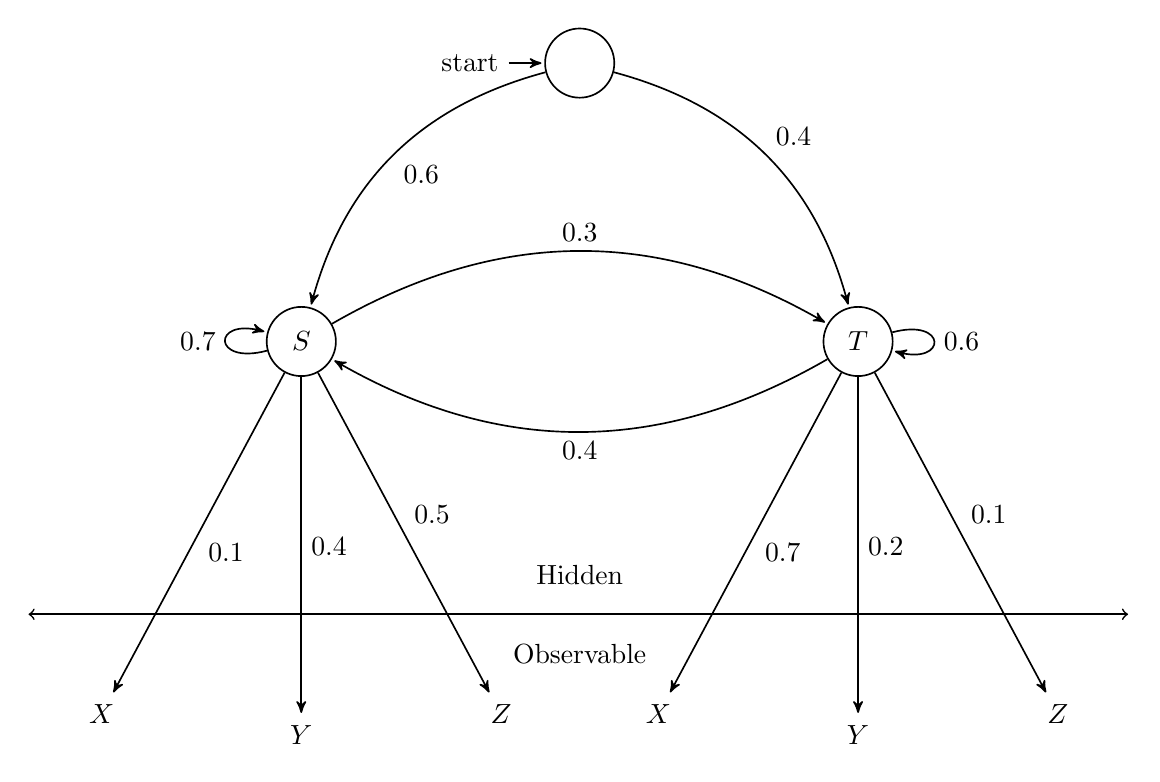
\begin{tikzpicture}[->,>=stealth',shorten >=1pt,auto,node distance=5cm,
		semithick]
										
		\node[initial,state] (I)                    {$$};
		\node[state]         (S) [below left of=I] {$S$};
		\node[state]         (T) [below right of=I] {$T$};
		\node[rectangle]         (SX) [below left of=S,yshift=-1.2cm,xshift=1cm]     {$X$};
		\node[rectangle]         (SY) [below of=S]     {$Y$};  
		\node[rectangle]         (SZ) [below right of=S,yshift=-1.2cm,xshift=-1cm]     {$Z$};
		\node[rectangle]         (TX) [below left of=T,yshift=-1.2cm,xshift=1cm]     {$X$};
		\node[rectangle]         (TY) [below of=T]     {$Y$};  
		\node[rectangle]         (TZ) [below right of=T,yshift=-1.2cm,xshift=-1cm]     {$Z$};  
										
		\path (I) edge [bend right]    node {0.6} (S)
		edge [bend left]     node {0.4} (T)
		(S) edge [loop left]    node {0.7} (S)
		edge [bend left]    node {0.3} (T)
		edge                node {0.1} (SX)
		edge                node {0.4} (SY)
		edge                node {0.5} (SZ)
		(T) edge [loop right]   node {0.6} (T)
		edge [bend left]    node {0.4} (S)
		edge                node {0.7} (TX)
		edge                node {0.2} (TY)
		edge                node {0.1} (TZ);   
		\draw [to-to] (-7,-7) -- (7,-7); 
		\node at (0, -6.5) {Hidden};
		\node at (0, -7.5) {Observable};                   
	\end{tikzpicture}
\end{center}

In this diagram, nodes $\{S, T\}$ represent the hidden states and $\{X, Y, Z\}$ represent observable states. The unlabelled node is the start node. These states together with the associated probabilities fully characterize the HMM. The state transition probabilites denoted by $A$ can be represented as,

\[
	A = \kbordermatrix{
		& S & T \\
		S & 0.7 & 0.3 \\
		T & 0.6 & 0.4 \\
	}
\]

The emmission probabilities are denoted by $B$.

\[
	B = \kbordermatrix{
		& X & Y & Z \\
		S & 0.1 & 0.4 & 0.5 \\
		T & 0.7 & 0.2 & 0.1 \\
	}
\]

Lastly, initial state distribution is denoted by $\pi$.

\[
	\pi = \kbordermatrix{
		& S & T \\
		& 0.6 & 0.4  
	}
\]

\section{The three problems of HMM}

\subsection{The Evaluation Problem}

Given a HMM, $\lambda=(A, B, \pi)$ and a set of observations $O$, find $P(O|\lambda)$ (probability that the observations were generated by the model).

Consider the HMM in the example above and let $O = (ZXY)$.

\begin{align*}
	P(ZXY|\lambda) & = P(SSS, ZXY|\lambda)  \\
	               & +\ P(SST, ZXY|\lambda) \\
	               & +\ P(STS, ZXY|\lambda) \\
	               & +\ P(STT, ZXY|\lambda) \\
	               & +\ P(TSS, ZXY|\lambda) \\
	               & +\ P(TST, ZXY|\lambda) \\
	               & +\ P(TTS, ZXY|\lambda) \\
	               & +\ P(TTT, ZXY|\lambda) \\  
\end{align*}

Each of the terms on R.H.S. can be calculated using the following law of probability.

\begin{align*}
	P(a, b|c) & = \frac{P(a, b, c) }{P(c)}                            \\ 
	          & = \frac{P(a, c) }{P(c)} * \frac{P(a, b, c) }{P(a, c)} \\
	          & = P(a|c) * P(b|a,c)                                   
\end{align*} 

\begin{table}[h!]
	\centering
	\caption{$P(ZXY|\lambda)$ calculation}
	\label{tab:table1}
	\begin{tabular}{cccc|c}
		\toprule
		HS  & OS  & $P(HS|\lambda)$   & $P(OS|HS, \lambda)$ & $P(HS, OS|\lambda)$ \\
		\midrule
		SSS & ZXY & 0.6*0.7*0.7=0.294 & 0.5*0.1*0.4=0.020   & 0.005880            \\
		SST & ZXY & 0.6*0.7*0.3=0.126 & 0.5*0.1*0.2=0.010   & 0.001260            \\
		STS & ZXY & 0.6*0.3*0.4=0.072 & 0.5*0.7*0.4=0.140   & 0.010080            \\
		STT & ZXY & 0.6*0.3*0.6=0.108 & 0.5*0.7*0.2=0.070   & 0.007560            \\
		TSS & ZXY & 0.4*0.4*0.7=0.112 & 0.1*0.1*0.4=0.004   & 0.000448            \\
		TST & ZXY & 0.4*0.4*0.3=0.048 & 0.1*0.1*0.2=0.002   & 0.000096            \\
		TTS & ZXY & 0.4*0.6*0.4=0.096 & 0.1*0.7*0.4=0.028   & 0.002688            \\
		TTT & ZXY & 0.4*0.6*0.6=0.144 & 0.1*0.7*0.2=0.014   & 0.002016            \\
		\midrule
		    &     &                   & $P(ZXY|\lambda)$    & 0.030028            \\
		\bottomrule
	\end{tabular}
\end{table}

Calculation in this manner is expensive because probabilities corresponding to all permutations of hidden states of the same length as the length of observed sequence have to be calculated. 

To visualize the above calculation, consider the following diagrammatic represntation.

\begin{center}
	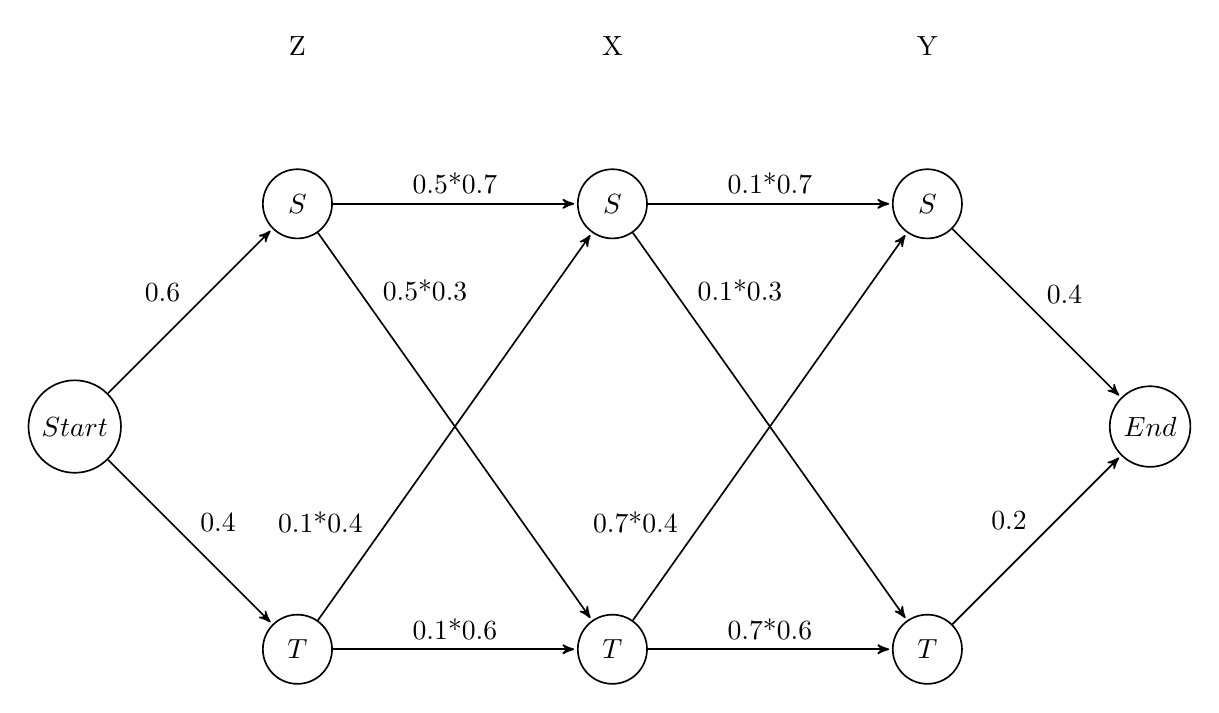
\begin{tikzpicture}[->,>=stealth',shorten >=1pt,auto,node distance=4cm,
		semithick]
										
		\node[state] (Start)                    {$Start$};
		\node[state] (S1) [above right of=Start] {$S$};
		\node[state] (T1) [below right of=Start] {$T$};
		\node[state] (S2) [right of=S1] {$S$};
		\node[state] (T2) [right of=T1] {$T$};
		\node[state] (S3) [right of=S2] {$S$};
		\node[state] (T3) [right of=T2] {$T$};
		\node[state] (End) [below right of=S3] {$End$};
		\node [rectangle, node distance=2cm] (Z) [above of=S1] {Z};
		\node [rectangle, node distance=2cm] (X) [above of=S2] {X};
		\node [rectangle, node distance=2cm] (Y) [above of=S3] {Y};						
										                
		\path (Start) edge  node {0.6} (S1)
		edge  node {0.4} (T1)
		(S1) edge  node {0.5*0.7} (S2)
		edge  node [pos=0.2] {0.5*0.3} (T2)
		(T1) edge  node [pos=0.2] {0.1*0.4} (S2)
		edge  node {0.1*0.6} (T2)
		(S2) edge  node {0.1*0.7} (S3)
		edge node [pos=0.2] {0.1*0.3} (T3)
		(T2) edge node [pos=0.2] {0.7*0.4} (S3)
		edge node {0.7*0.6} (T3)
		(S3) edge node {0.4} (End)
		(T3) edge node {0.2} (End);                     
	\end{tikzpicture}
\end{center}

The arrow from $S$ under $Z$ and $S$ under $X$ is labelled 0.5*0.7 as probability of emitting $Z$ given $S$ is 0.5 and probability of transition from $S$ to $S$ is 0.7. The arrow from $Start$ to $S$ is labelled 0.6 as initial probability of transitioning to $S$ is 0.6. Similarly, the arrow from $S$ to End is labelled 0.4 as probability of emitting $Y$ given $S$ is 0.4.

Every path in the diagram from $Start$ to $End$ has a special meaning in the sense that the multiplication of all labels on the path (which henceforth shall be called its value) is equal to the joint probability of the observation sequence and the hidden state transition sequence defined by the path given the model.

The diagram also leads to the fact that $P(ZXY|\lambda)$ can be thought of as arising out of the enumeration of all paths from $Start$ to $End$ and then summation over their value. 

Dynamic Programming can be used to circumvent enumeration and speed up the computation as shown below,


\begin{center}
	\begin{tikzpicture}[->,>=stealth',shorten >=1pt,auto,node distance=4cm,
		semithick]
										
		\node[state] (Start)                    {$1$};
		\node[state] (S1) [above right of=Start] {$0.6$};
		\node[rectangle, node distance=2cm] (D1) [right of=S1] {$=1*0.6$};
		\node[state] (T1) [below right of=Start] {$0.4$};
		\node[rectangle, node distance=2cm] (D2) [right of=T1] {$=1*0.4$};		 
		\path (Start) edge  node {0.6} (S1)
		edge  node {0.4} (T1);                     
	\end{tikzpicture}
\end{center}

\noindent\rule{\textwidth}{0.6pt}

\begin{center}
	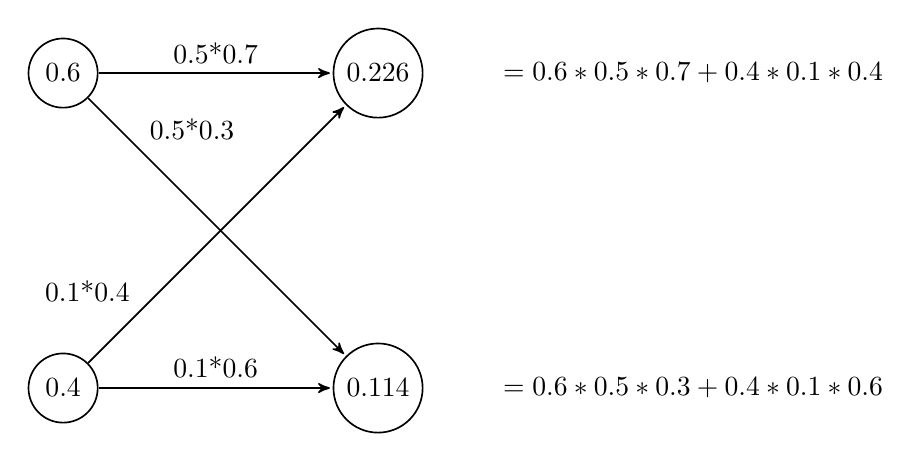
\begin{tikzpicture}[->,>=stealth',shorten >=1pt,auto,node distance=4cm,
		semithick]
										
		\node[state] (S1) {$0.6$};
		\node[state] (T1) [below of=S1] {$0.4$};
		\node[state] (S2) [right of=S1] {$0.226$};
		\node[rectangle, node distance=4cm] (D2) [right of=S2] {$=0.6*0.5*0.7 + 0.4*0.1*0.4$};	
		\node[state] (T2) [right of=T1] {$0.114$};
		\node[rectangle, node distance=4cm] (D2) [right of=T2] {$=0.6*0.5*0.3 + 0.4*0.1*0.6$};				
							                
		\path 
		(S1) edge  node {0.5*0.7} (S2)
		edge  node [pos=0.2] {0.5*0.3} (T2)
		(T1) edge  node [pos=0.2] {0.1*0.4} (S2)
		edge  node {0.1*0.6} (T2);		
	\end{tikzpicture}
\end{center}

\noindent\rule{\textwidth}{0.6pt}

\begin{center}
	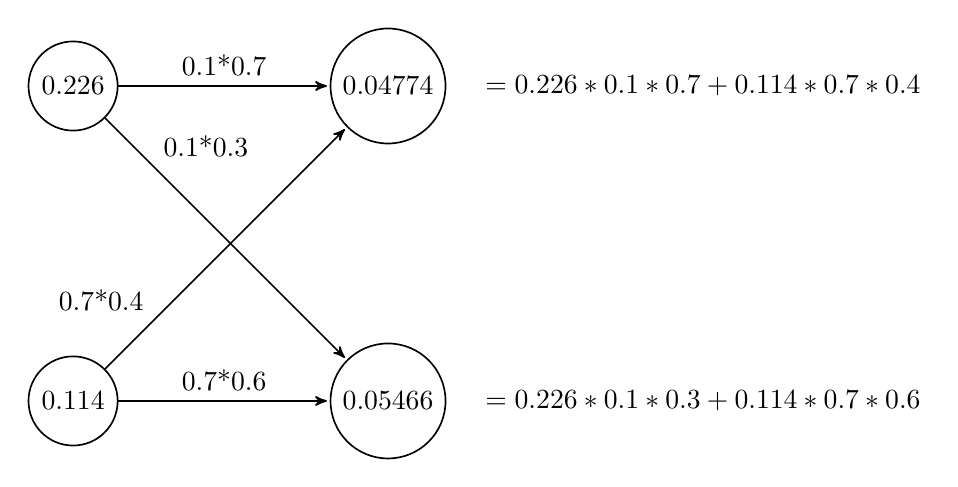
\begin{tikzpicture}[->,>=stealth',shorten >=1pt,auto,node distance=4cm,
		semithick]
										
		\node[state] (S2) {$0.226$};
		\node[state] (T2) [below of=S2] {$0.114$};
		\node[state] (S3) [right of=S2] {$0.04774$};
		\node[rectangle, node distance=4cm] (D3) [right of=S3] {$=0.226*0.1*0.7 + 0.114*0.7*0.4$};
		\node[state] (T3) [right of=T2] {$0.05466$};
		\node[rectangle, node distance=4cm] (D3) [right of=T3] {$=0.226*0.1*0.3 + 0.114*0.7*0.6$};
									
										                
		\path 
		(S2) edge  node {0.1*0.7} (S3)
		edge node [pos=0.2] {0.1*0.3} (T3)
		(T2) edge node [pos=0.2] {0.7*0.4} (S3)
		edge node {0.7*0.6} (T3);                     
	\end{tikzpicture}
\end{center}

\noindent\rule{\textwidth}{0.6pt}

\begin{center}
	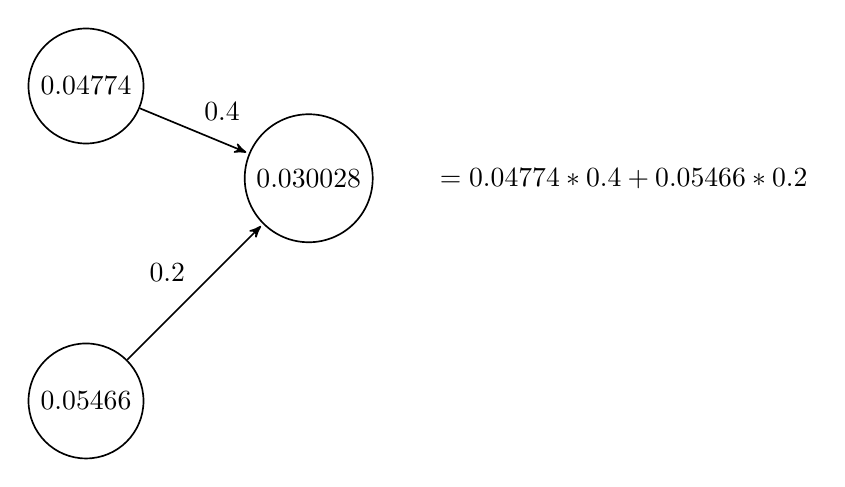
\begin{tikzpicture}[->,>=stealth',shorten >=1pt,auto,node distance=4cm,
		semithick]
										
		\node[state] (S3) {$0.04774$};
		\node[state] (T3) [below of=S3] {$0.05466$};
		\node[state] (End) [above right of=T3] {$0.030028$};
		\node[rectangle, node distance=4cm] (D4) [right of=End] {$=0.04774*0.4 + 0.05466*0.2$};				                
		\path 
		(S3) edge node {0.4} (End)
		(T3) edge node {0.2} (End);                     
	\end{tikzpicture}
\end{center}

In this algorithm, each node on the right keeps track of sum of values of all paths from $Start$ to that node denoted by $\alpha_t(state)$.

\begin{table}[h!]
	\centering
	\begin{tabular}{c|c|c|c}
		\toprule
		              & $t=1$ & $t=2$ & $t=3$   \\
		\midrule
		$\alpha_t(S)$ & 0.6   & 0.226 & 0.04774 \\
		$\alpha_t(T)$ & 0.4   & 0.114 & 0.05466 \\
		\bottomrule
	\end{tabular}
\end{table}

The same algorithm can be run backwards from the $End$ node and work its way towards the $Start$ node. Now, each node in the left will keep track of sum of values of all paths from $End$ to that node denoted by $\beta_t(state)$.

\begin{table}[h!]
	\centering
	\begin{tabular}{c|c|c|c}
		\toprule
		             & $t=1$   & $t=2$ & $t=3$ \\
		\midrule
		$\beta_t(S)$ & 0.0413  & 0.034 & 0.4   \\
		$\beta_t(T)$ & 0.01312 & 0.196 & 0.2   \\
		\bottomrule
	\end{tabular}
\end{table}

It is apparent that the following relation must hold,

\begin{align*}
	\sum_{\text{all states}} \alpha_t(state)*\beta_t(state) = 0.030028\  \forall\ t 
\end{align*}
 
\subsection{The Decoding Problem}

Given a HMM, $\lambda = (A, B, \pi)$ and a set of observations $O$, find the most likely sequence of hidden states that led the model to emit $O
$. The solution to this is straightforward. At each time step, the state corrresponding to maximum value of $\alpha_t(state)*\beta_t(state)$ is chosen.

\begin{table}[h!]
	\centering
	\caption{Decoding solution}
	\label{tab:table2}
	\begin{tabular}{c|c|c|c}
		\toprule
		             & $t=1$       & $t=2$       & $t=3$       \\
		\midrule
		S            & 0.6*0.0413  & 0.226*0.034 & 0.04774*0.4 \\
		T            & 0.4*0.01312 & 0.114*0.196 & 0.05466*0.2 \\
		\midrule
		Chosen State & S           & T           & S           \\
		\bottomrule
	\end{tabular}
\end{table}

\subsection{The Learning Problem}

If only the observation sequence $O$ were given, how can one estimate $\lambda$? Make a good guess of the number of hidden states and follow:

\begin{enumerate}
	\item Non uniformly initialize a model $\lambda = (A, B, \pi)$.
	\item Compute $\alpha_t(state)$ and $\beta_t(state)$ for all times and states using the solution to Problem 1.
	\item Re-estimate the model $\lambda$.
	\item Go to step 2 if $P(O|\lambda)$ increases reasonably or if out of iterations. 
\end{enumerate}

The only question that remains is: How to re-estimate $\lambda$?

\begin{center}
	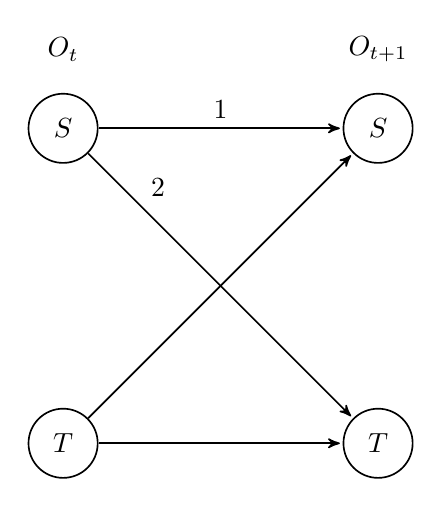
\begin{tikzpicture}[->,>=stealth',shorten >=1pt,auto,node distance=4cm,
		semithick]
										
		\node[state] (S1) {$S$};
		\node[] (O1) [above of=S1, node distance=1cm]{$O_t$};
		\node[state] (T1) [below of=S1] {$T$};	
		\node[state] (S2) [right of=S1] {$S$};	
		\node[] (O2) [above of=S2, node distance=1cm]{$O_{t+1}$};		
		\node[state] (T2) [right of=T1] {$T$};				
							                
		\path 
		(S1) edge  node {1} (S2)
		edge  node [pos=0.2] {2} (T2)
		(T1) edge  node [pos=0.2] {} (S2)
		edge  node {} (T2);		
	\end{tikzpicture}
\end{center}

Remember that $P(O|\lambda)$ is the sum of values if all paths from $Start$ to $End$. A fraction of $P(O|\lambda)$ comes from the sum of values of all paths that contain transtion $(state_t =S \rightarrow state_{t+1}=S)$ labelled by $1$ in the above figure. Denote it by $\gamma_t(S \rightarrow S)$.

A yet another fraction comes from the sum of values of all paths that contain transtion $(state_t =S \rightarrow state_{t+1}=T)$ labelled by $2$ denoted by $\gamma_t(S \rightarrow T)$. Also let, 
\begin{align*}
	\gamma_t(S) = \gamma_t(S \rightarrow S) + \gamma_t(S \rightarrow T) 
\end{align*}

Is $\frac{\gamma_t(S \rightarrow S)}{\gamma_t(S)}$ a good estimate of $A(S \rightarrow S)$? Kind of. But remember that only one time $t$ is considered. A better estimate would be,

\begin{align*}
	A(S \rightarrow S) \approx \frac{\sum_t \gamma_t(S \rightarrow S)}{\sum_t \gamma_t(S)} 
\end{align*} 

Similarly, $B(S \rightarrow OS)$ is estimated by,

\begin{align*}
	B(S \rightarrow OS) \approx \frac{\sum_{t|O_t = OS} \gamma_t(S)}{\sum_t \gamma_t(S)} 
\end{align*} 

This completes the discussion of the solution to the learning problem in HMMs.

\end{document}